\subsection{Velocità della luce}

Si vuole utilizzare l'apparato a disposizione per misurare la velocità della luce. Si noti che con tale apparato è possibile misurare solamente differenze di tempi
e non tempi assoluti (vista tutta l'elettronica utilizzata). Le misure sono state prese come descritto nell'analisi dati, e a disposizione quindi si hanno:
\begin{itemize}
\item la distanza tra i due rivelatori
\item i diversi ritardi nella rivelazione nelle due diverse configurazioni
\item le dimensioni del piombo contenente la sorgente
\item il datasheet dei rivelatori
\end{itemize}
Si cerchi una formula per ricavare la velocità della luce date queste informazioni. Il ragionamento farà uso di due approssimazioni: la sorgente è puntiforme lungo la direzione
di volo dei fotoni rivelati (assumibile in quanto consisteva in un disco posto in maniera perpendicolare a tale direzione)
e si può pensare il fotone venga rivelato sempre nella stessa posizione dentro il rivelatore.\\

Con tali ipotesi, si considerino le misure di lunghezze con la seguente notazione:
\begin{itemize}
\item $R_1$ indica lo spazio medio percorso dai fotoni nel rivelatore prima di interagire con lo stesso
\item $x_1$ indica la distanza tra la placca in piombo più vicina e il rivelatore 1
\item $\delta_1$ indica lo spessore della placca in piombo più vicina al rivelatore 1
\end{itemize}
E analoga notazione per quanto riguarda il rivelatore 2. In poche parole le ipotesi fatte consistono nel fatto che $R_1=R_2$ e che questi valori si possono prendere
come esatti.\footnote{In realtà, questa ipotesi viene verificata nel limite delle infinite misure; dato che il campione preso è sufficientemente grande, si suppone essa sia
valida}\\
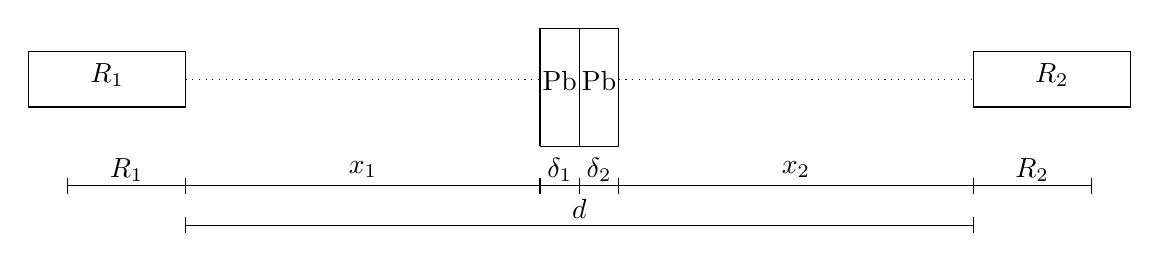
\begin{tikzpicture}
%\draw[->,thick] (-4,0)--(4,0) node[right]{$z$};

%\node [label=below:-e,draw,fill=black,circle,inner sep=0pt,minimum size=3pt] at (-3,0) {};
%\node [label=below:+e,draw,fill=black,circle,inner sep=0pt,minimum size=3pt] at (-2,0) {};
%\node [label=below:+e,draw,fill=black,circle,inner sep=0pt,minimum size=3pt] at (2,0) {};
%\node [label=below:-e,draw,fill=black,circle,inner sep=0pt,minimum size=3pt] at (3,0) {};


\draw[] (-4,0)--(-4,0.7)--(-2,0.7)--(-2,0)--(-4,0) node[label=above:$R_1$, black, midway, yshift=0.3]{}; %primo rivelatore
\draw[] (8,0)--(8,0.7)--(10,0.7)--(10,0)--(8,0) node[label=above:$R_2$, black, midway, yshift=0.3]{}; %secondo rivelatore

\draw[] (2.5,-0.5)--(2.5,1)--(3,1)--(3,-0.5)--(2.5,-0.5) node[label=above:Pb, black, midway, yshift=13]{}; %primo piombo
\draw[] (3,-0.5)--(3,1)--(3.5,1)--(3.5,-0.5)--(3,-0.5) node[label=above:Pb, black, midway, yshift=13]{}; %secondo piombo

%\node[starburst, minimum width=3cm, minimum height=2cm,line width=1.5pt]{};

\draw[] (-3.5,-1)--(9.5,-1) node[right]{};

\draw[] (-3.5,-1.1)--(-3.5,-0.9){};
\draw[] (-2,-1.1)--(-2,-0.9){};
\draw[] (2.5,-1.1)--(2.5,-0.9){};
\draw[] (3,-1.1)--(3,-0.9){};
\draw[] (3.5,-1.1)--(3.5,-0.9){};
\draw[] (8,-1.1)--(8,-0.9){};
\draw[] (9.5,-1.1)--(9.5,-0.9){};

\node[] at (-2.75,-0.8) {$R_1$};
\node[] at (0.25,-0.8) {$x_1$};
\node[] at (2.75,-0.8) {$\delta_1$};
\node[] at (3.25,-0.8) {$\delta_2$};
\node[] at (5.75,-0.8) {$x_2$};
\node[] at (8.75,-0.8) {$R_2$};

\draw[dotted](-2,0.35)--(2.5,0.35){};
\draw[dotted](3.5,0.35)--(8,0.35){};

\draw[] (-2,-1.5)--(8,-1.5) node[right]{};
\node[] at (3,-1.3) {$d$};
\draw[] (-2,-1.6)--(-2,-1.4){};
\draw[] (8,-1.6)--(8,-1.4){};


%\draw [decorate,decoration={brace,amplitude=10pt},xshift=0pt,yshift=0pt] (-3,0) -- (-2,0) node [label=above:$z_2$,black,midway,yshift=0.2cm] {};
%\draw [decorate,decoration={brace,amplitude=10pt},xshift=0pt,yshift=0pt] (-2,0) -- (2,0) node [label=above:$R$,black,midway,yshift=0.2cm] {};
%\draw [decorate,decoration={brace,amplitude=10pt},xshift=0pt,yshift=0pt] (2,0) -- (3,0) node [label=above:$z_1$,black,midway,yshift=0.2cm] {};

\end{tikzpicture} 


A questo punto, se la configurazione è la A, si possono descrivere i tempi di percorrenza dei fotoni prima che vengano rivelati come\footnote:
$$
  t_{1A} = \frac{\delta_1 + nR_1}{c} \hspace{2cm} t_{2A} = \frac{\delta_2 + x_2 + nR_2}{c}
$$
Ove $n$ indica il coefficiente di rigrazione all'interno del rivelatore stesso. Quindi il TAC rivelerà l'intervallo temporale:
$$
  \delta t_A = t_{2A} - t_{1A} = \frac{\delta_2 + x_2 + nR_2-\delta_1-nR_1}{c}
$$
Analogamente per la configurazione B si trova:
$$
  t_{1B} = \frac{\delta_1 + x_1 + nR_1}{c} \hspace{2cm} t_{2B} = \frac{\delta_2 + nR_2}{c}
$$
e l'intervallo rilevato dal TAC sarà:
$$
  \Delta t_B = t_{2B} - t_{1B} = \frac{\delta_2 + nR_2 - \delta_1 - x_1 - nR_1}{c}
$$
A questo punto, però, questi due intervalli non hanno senso presi singolarmente, in quanto non rivelano effettivamente un intervallo temporale ma il tempo riferito ad
uno zero che, sebbene non sia noto oggettivamente, è lo stesso per entrambe le misure (infatti non si è toccato l'apparato strumentale se non per spostare la sorgente
racchiusa tra le placche di piombo). Perciò ha senso fisico la loro differenza, che si può stimare con facilità:
$$
  \Delta t = \Delta t_A - \Delta t_B = \frac{{\delta_2 + x_2 + nR_2 - \delta_1 - nR_1}{-\delta_2 - nR_2 + \delta_1 + x_1 + nR_1}}{c} = \frac{x_1 + x_2}{c}
$$
Perciò per stimare la velocità della luce è sufficiente andare a misurare la distanza dei due rivelatori a meno delle placche di piombo e la distanza temporale tra i due
picchi nei grafici calibrati del TAC. Però, in sede di esecuzione dell'esperimento, non si è effettivamente misurata quella distanza ma solamente le distanze tra la sorgente
e i rivelatori nelle due configurazioni, quindi si ha una stima di $\delta$ e una stima di $ 2 * \delta + x$ per i due casi.\\

Si venga alla vera e propria analisi dati: si vuole applicare la formula, appena dimostrata:
$$
  c = \frac{x_1+x_2}{\Delta t}
$$
si ragioni sul numeratore, cioè la misura di lunghezza: si conoscono i valori, misurati con il metro:
$$
  d = 173.2 cm \hspace{2cm} \delta = 3.7 cm
$$
ove d indica la distanza tra i due rivelatori e $\delta$ indica le misure (uguali) dei blocchi di piombo.
Ora si è interessati a $x_1+x_2$, per motivi geometrici si può riscrivere in funzione delle variabili misurate come:
$$
  x_1+x_2 = 2 ( d - 2 \delta)
$$
Come errore sulle variabili si considera un errore triangolare associato al fatto che il metro aveva una scala dei millimetri, quindi si ha
$$
  \sigma_d = \sigma_\delta = \frac{0.5\text{mm}}{\sqrt6} = 0.2 mm
$$
\\

SOra si pensi al denominatore dell'equazione per la velocità della luce, cioè la differenza tra le distanze temporali nelle due diverse configurazioni dell'esperimento.
Si riscriva tenendo conto della calibrazione:
$$
  \Delta t = \Delta t_A - \Delta t_B = m\Delta t_A + q - m\Delta t_B - q = m (\Delta t_A - \Delta t_B) 
$$
Ove $m,q$, sono i coefficienti della calibrazione stimati nelle sezioni precedenti. I due picchi si possono vedere, già calibrati, nella figura sottostante.\\
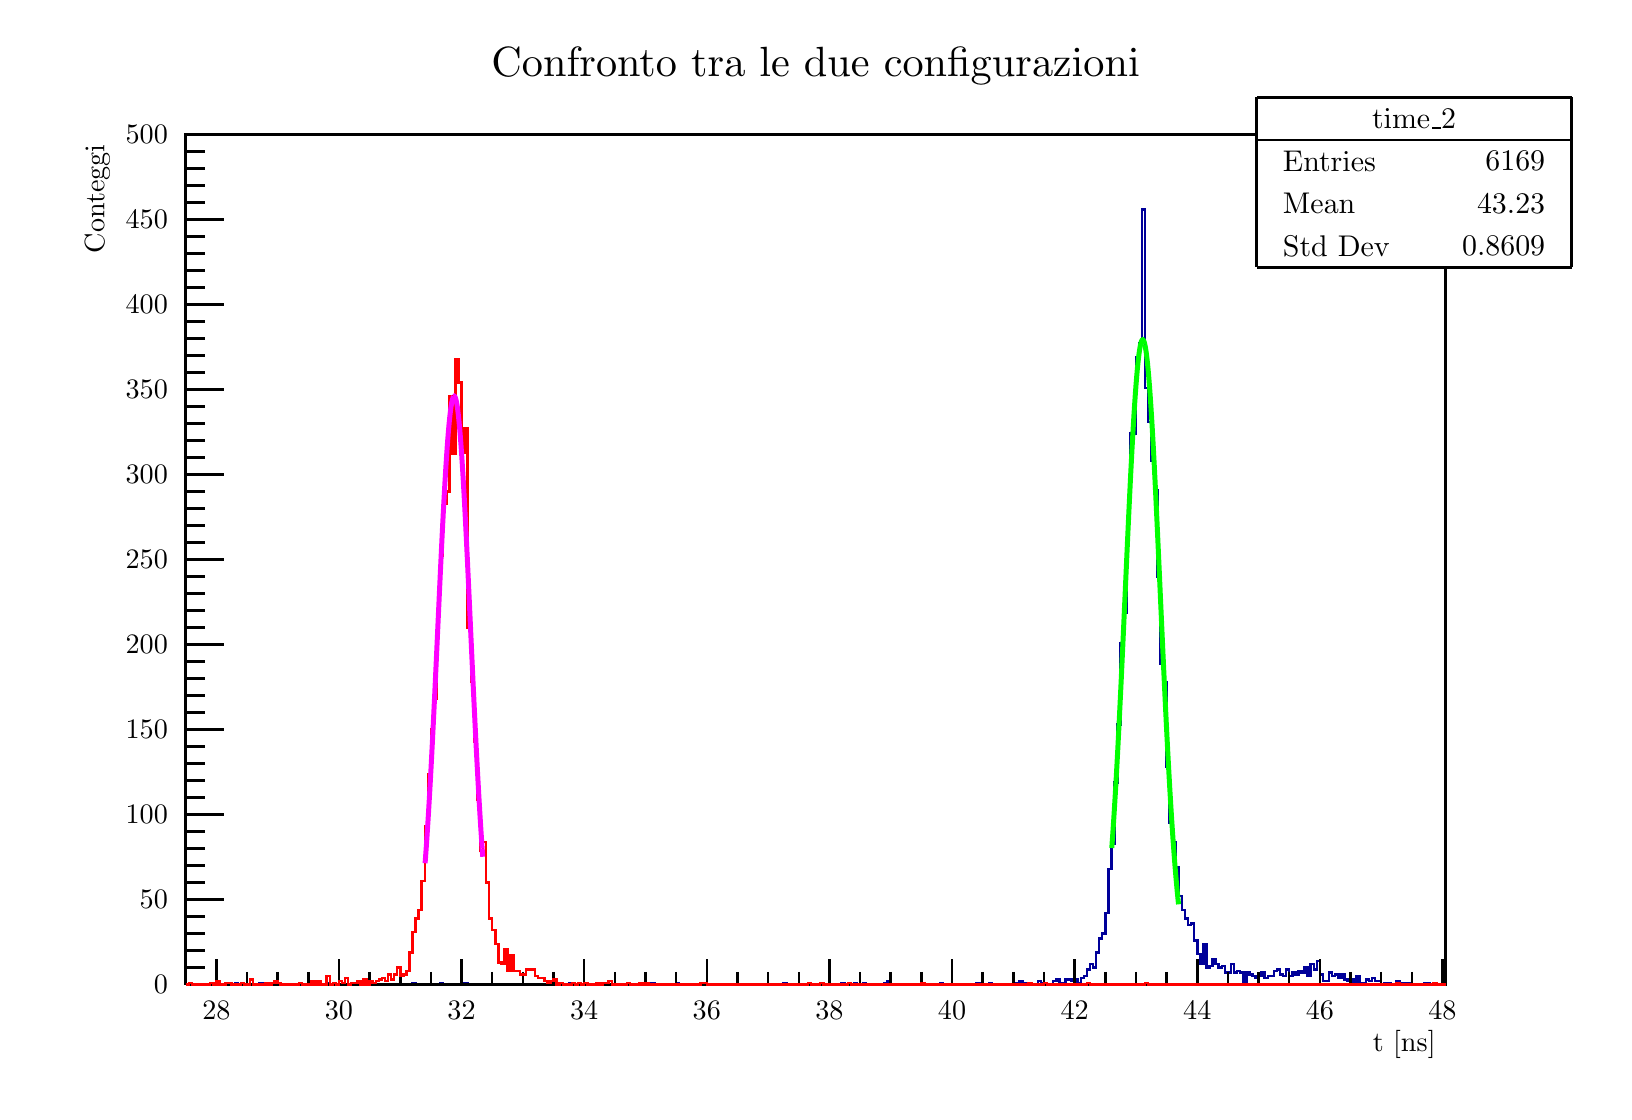
\begin{tikzpicture}
\pgfdeclareplotmark{cross} {
\pgfpathmoveto{\pgfpoint{-0.3\pgfplotmarksize}{\pgfplotmarksize}}
\pgfpathlineto{\pgfpoint{+0.3\pgfplotmarksize}{\pgfplotmarksize}}
\pgfpathlineto{\pgfpoint{+0.3\pgfplotmarksize}{0.3\pgfplotmarksize}}
\pgfpathlineto{\pgfpoint{+1\pgfplotmarksize}{0.3\pgfplotmarksize}}
\pgfpathlineto{\pgfpoint{+1\pgfplotmarksize}{-0.3\pgfplotmarksize}}
\pgfpathlineto{\pgfpoint{+0.3\pgfplotmarksize}{-0.3\pgfplotmarksize}}
\pgfpathlineto{\pgfpoint{+0.3\pgfplotmarksize}{-1.\pgfplotmarksize}}
\pgfpathlineto{\pgfpoint{-0.3\pgfplotmarksize}{-1.\pgfplotmarksize}}
\pgfpathlineto{\pgfpoint{-0.3\pgfplotmarksize}{-0.3\pgfplotmarksize}}
\pgfpathlineto{\pgfpoint{-1.\pgfplotmarksize}{-0.3\pgfplotmarksize}}
\pgfpathlineto{\pgfpoint{-1.\pgfplotmarksize}{0.3\pgfplotmarksize}}
\pgfpathlineto{\pgfpoint{-0.3\pgfplotmarksize}{0.3\pgfplotmarksize}}
\pgfpathclose
\pgfusepathqstroke
}
\pgfdeclareplotmark{cross*} {
\pgfpathmoveto{\pgfpoint{-0.3\pgfplotmarksize}{\pgfplotmarksize}}
\pgfpathlineto{\pgfpoint{+0.3\pgfplotmarksize}{\pgfplotmarksize}}
\pgfpathlineto{\pgfpoint{+0.3\pgfplotmarksize}{0.3\pgfplotmarksize}}
\pgfpathlineto{\pgfpoint{+1\pgfplotmarksize}{0.3\pgfplotmarksize}}
\pgfpathlineto{\pgfpoint{+1\pgfplotmarksize}{-0.3\pgfplotmarksize}}
\pgfpathlineto{\pgfpoint{+0.3\pgfplotmarksize}{-0.3\pgfplotmarksize}}
\pgfpathlineto{\pgfpoint{+0.3\pgfplotmarksize}{-1.\pgfplotmarksize}}
\pgfpathlineto{\pgfpoint{-0.3\pgfplotmarksize}{-1.\pgfplotmarksize}}
\pgfpathlineto{\pgfpoint{-0.3\pgfplotmarksize}{-0.3\pgfplotmarksize}}
\pgfpathlineto{\pgfpoint{-1.\pgfplotmarksize}{-0.3\pgfplotmarksize}}
\pgfpathlineto{\pgfpoint{-1.\pgfplotmarksize}{0.3\pgfplotmarksize}}
\pgfpathlineto{\pgfpoint{-0.3\pgfplotmarksize}{0.3\pgfplotmarksize}}
\pgfpathclose
\pgfusepathqfillstroke
}
\pgfdeclareplotmark{newstar} {
\pgfpathmoveto{\pgfqpoint{0pt}{\pgfplotmarksize}}
\pgfpathlineto{\pgfqpointpolar{44}{0.5\pgfplotmarksize}}
\pgfpathlineto{\pgfqpointpolar{18}{\pgfplotmarksize}}
\pgfpathlineto{\pgfqpointpolar{-20}{0.5\pgfplotmarksize}}
\pgfpathlineto{\pgfqpointpolar{-54}{\pgfplotmarksize}}
\pgfpathlineto{\pgfqpointpolar{-90}{0.5\pgfplotmarksize}}
\pgfpathlineto{\pgfqpointpolar{234}{\pgfplotmarksize}}
\pgfpathlineto{\pgfqpointpolar{198}{0.5\pgfplotmarksize}}
\pgfpathlineto{\pgfqpointpolar{162}{\pgfplotmarksize}}
\pgfpathlineto{\pgfqpointpolar{134}{0.5\pgfplotmarksize}}
\pgfpathclose
\pgfusepathqstroke
}
\pgfdeclareplotmark{newstar*} {
\pgfpathmoveto{\pgfqpoint{0pt}{\pgfplotmarksize}}
\pgfpathlineto{\pgfqpointpolar{44}{0.5\pgfplotmarksize}}
\pgfpathlineto{\pgfqpointpolar{18}{\pgfplotmarksize}}
\pgfpathlineto{\pgfqpointpolar{-20}{0.5\pgfplotmarksize}}
\pgfpathlineto{\pgfqpointpolar{-54}{\pgfplotmarksize}}
\pgfpathlineto{\pgfqpointpolar{-90}{0.5\pgfplotmarksize}}
\pgfpathlineto{\pgfqpointpolar{234}{\pgfplotmarksize}}
\pgfpathlineto{\pgfqpointpolar{198}{0.5\pgfplotmarksize}}
\pgfpathlineto{\pgfqpointpolar{162}{\pgfplotmarksize}}
\pgfpathlineto{\pgfqpointpolar{134}{0.5\pgfplotmarksize}}
\pgfpathclose
\pgfusepathqfillstroke
}
\definecolor{c}{rgb}{1,1,1};
\draw [color=c, fill=c] (0,0) rectangle (20,13.4957);
\draw [color=c, fill=c] (2,1.34957) rectangle (18,12.1461);
\definecolor{c}{rgb}{0,0,0};
\draw [c,line width=0.9] (2,1.34957) -- (2,12.1461) -- (18,12.1461) -- (18,1.34957) -- (2,1.34957);
\definecolor{c}{rgb}{1,1,1};
\draw [color=c, fill=c] (2,1.34957) rectangle (18,12.1461);
\definecolor{c}{rgb}{0,0,0};
\draw [c,line width=0.9] (2,1.34957) -- (2,12.1461) -- (18,12.1461) -- (18,1.34957) -- (2,1.34957);
\definecolor{c}{rgb}{0,0,0.6};
\draw [c,line width=0.9] (2,1.34957) -- (2.03893,1.34957) -- (2.03893,1.34957) -- (2.07786,1.34957) -- (2.07786,1.34957) -- (2.11679,1.34957) -- (2.11679,1.34957) -- (2.15572,1.34957) -- (2.15572,1.34957) -- (2.19465,1.34957) -- (2.19465,1.34957) --
 (2.23358,1.34957) -- (2.23358,1.34957) -- (2.27251,1.34957) -- (2.27251,1.34957) -- (2.31144,1.34957) -- (2.31144,1.34957) -- (2.35037,1.34957) -- (2.35037,1.34957) -- (2.38929,1.34957) -- (2.38929,1.34957) -- (2.42822,1.34957) -- (2.42822,1.34957)
 -- (2.46715,1.34957) -- (2.46715,1.34957) -- (2.50608,1.34957) -- (2.50608,1.34957) -- (2.54501,1.34957) -- (2.54501,1.34957) -- (2.58394,1.34957) -- (2.58394,1.34957) -- (2.62287,1.34957) -- (2.62287,1.37116) -- (2.6618,1.37116) -- (2.6618,1.34957)
 -- (2.70073,1.34957) -- (2.70073,1.37116) -- (2.73966,1.37116) -- (2.73966,1.34957) -- (2.77859,1.34957) -- (2.77859,1.34957) -- (2.81752,1.34957) -- (2.81752,1.34957) -- (2.85645,1.34957) -- (2.85645,1.34957) -- (2.89538,1.34957) --
 (2.89538,1.34957) -- (2.93431,1.34957) -- (2.93431,1.37116) -- (2.97324,1.37116) -- (2.97324,1.34957) -- (3.01217,1.34957) -- (3.01217,1.34957) -- (3.0511,1.34957) -- (3.0511,1.34957) -- (3.09002,1.34957) -- (3.09002,1.34957) -- (3.12895,1.34957) --
 (3.12895,1.34957) -- (3.16788,1.34957) -- (3.16788,1.34957) -- (3.20681,1.34957) -- (3.20681,1.34957) -- (3.24574,1.34957) -- (3.24574,1.34957) -- (3.28467,1.34957) -- (3.28467,1.34957) -- (3.3236,1.34957) -- (3.3236,1.34957) -- (3.36253,1.34957) --
 (3.36253,1.34957) -- (3.40146,1.34957) -- (3.40146,1.34957) -- (3.44039,1.34957) -- (3.44039,1.34957) -- (3.47932,1.34957) -- (3.47932,1.34957) -- (3.51825,1.34957) -- (3.51825,1.34957) -- (3.55718,1.34957) -- (3.55718,1.34957) -- (3.59611,1.34957)
 -- (3.59611,1.34957) -- (3.63504,1.34957) -- (3.63504,1.34957) -- (3.67397,1.34957) -- (3.67397,1.34957) -- (3.7129,1.34957) -- (3.7129,1.34957) -- (3.75182,1.34957) -- (3.75182,1.34957) -- (3.79075,1.34957) -- (3.79075,1.37116) -- (3.82968,1.37116)
 -- (3.82968,1.34957) -- (3.86861,1.34957) -- (3.86861,1.34957) -- (3.90754,1.34957) -- (3.90754,1.34957) -- (3.94647,1.34957) -- (3.94647,1.34957) -- (3.9854,1.34957) -- (3.9854,1.34957) -- (4.02433,1.34957) -- (4.02433,1.34957) -- (4.06326,1.34957)
 -- (4.06326,1.34957) -- (4.10219,1.34957) -- (4.10219,1.34957) -- (4.14112,1.34957) -- (4.14112,1.34957) -- (4.18005,1.34957) -- (4.18005,1.34957) -- (4.21898,1.34957) -- (4.21898,1.34957) -- (4.25791,1.34957) -- (4.25791,1.34957) --
 (4.29684,1.34957) -- (4.29684,1.34957) -- (4.33577,1.34957) -- (4.33577,1.34957) -- (4.3747,1.34957) -- (4.3747,1.34957) -- (4.41363,1.34957) -- (4.41363,1.34957) -- (4.45255,1.34957) -- (4.45255,1.34957) -- (4.49148,1.34957) -- (4.49148,1.34957) --
 (4.53041,1.34957) -- (4.53041,1.34957) -- (4.56934,1.34957) -- (4.56934,1.34957) -- (4.60827,1.34957) -- (4.60827,1.34957) -- (4.6472,1.34957) -- (4.6472,1.34957) -- (4.68613,1.34957) -- (4.68613,1.34957) -- (4.72506,1.34957) -- (4.72506,1.34957) --
 (4.76399,1.34957) -- (4.76399,1.34957) -- (4.80292,1.34957) -- (4.80292,1.34957) -- (4.84185,1.34957) -- (4.84185,1.34957) -- (4.88078,1.34957) -- (4.88078,1.37116) -- (4.91971,1.37116) -- (4.91971,1.34957) -- (4.95864,1.34957) -- (4.95864,1.34957)
 -- (4.99757,1.34957) -- (4.99757,1.34957) -- (5.0365,1.34957) -- (5.0365,1.34957) -- (5.07543,1.34957) -- (5.07543,1.34957) -- (5.11436,1.34957) -- (5.11436,1.34957) -- (5.15328,1.34957) -- (5.15328,1.34957) -- (5.19221,1.34957) -- (5.19221,1.34957)
 -- (5.23114,1.34957) -- (5.23114,1.37116) -- (5.27007,1.37116) -- (5.27007,1.34957) -- (5.309,1.34957) -- (5.309,1.34957) -- (5.34793,1.34957) -- (5.34793,1.34957) -- (5.38686,1.34957) -- (5.38686,1.34957) -- (5.42579,1.34957) -- (5.42579,1.34957)
 -- (5.46472,1.34957) -- (5.46472,1.34957) -- (5.50365,1.34957) -- (5.50365,1.37116) -- (5.54258,1.37116) -- (5.54258,1.37116) -- (5.58151,1.37116) -- (5.58151,1.34957) -- (5.62044,1.34957) -- (5.62044,1.34957) -- (5.65937,1.34957) --
 (5.65937,1.34957) -- (5.6983,1.34957) -- (5.6983,1.34957) -- (5.73723,1.34957) -- (5.73723,1.34957) -- (5.77616,1.34957) -- (5.77616,1.34957) -- (5.81509,1.34957) -- (5.81509,1.34957) -- (5.85401,1.34957) -- (5.85401,1.34957) -- (5.89294,1.34957) --
 (5.89294,1.34957) -- (5.93187,1.34957) -- (5.93187,1.34957) -- (5.9708,1.34957) -- (5.9708,1.34957) -- (6.00973,1.34957) -- (6.00973,1.34957) -- (6.04866,1.34957) -- (6.04866,1.34957) -- (6.08759,1.34957) -- (6.08759,1.34957) -- (6.12652,1.34957) --
 (6.12652,1.34957) -- (6.16545,1.34957) -- (6.16545,1.34957) -- (6.20438,1.34957) -- (6.20438,1.34957) -- (6.24331,1.34957) -- (6.24331,1.34957) -- (6.28224,1.34957) -- (6.28224,1.34957) -- (6.32117,1.34957) -- (6.32117,1.34957) -- (6.3601,1.34957)
 -- (6.3601,1.34957) -- (6.39903,1.34957) -- (6.39903,1.34957) -- (6.43796,1.34957) -- (6.43796,1.34957) -- (6.47689,1.34957) -- (6.47689,1.34957) -- (6.51582,1.34957) -- (6.51582,1.34957) -- (6.55474,1.34957) -- (6.55474,1.34957) --
 (6.59367,1.34957) -- (6.59367,1.34957) -- (6.6326,1.34957) -- (6.6326,1.34957) -- (6.67153,1.34957) -- (6.67153,1.34957) -- (6.71046,1.34957) -- (6.71046,1.34957) -- (6.74939,1.34957) -- (6.74939,1.34957) -- (6.78832,1.34957) -- (6.78832,1.34957) --
 (6.82725,1.34957) -- (6.82725,1.34957) -- (6.86618,1.34957) -- (6.86618,1.37116) -- (6.90511,1.37116) -- (6.90511,1.34957) -- (6.94404,1.34957) -- (6.94404,1.34957) -- (6.98297,1.34957) -- (6.98297,1.34957) -- (7.0219,1.34957) -- (7.0219,1.34957) --
 (7.06083,1.34957) -- (7.06083,1.34957) -- (7.09976,1.34957) -- (7.09976,1.34957) -- (7.13869,1.34957) -- (7.13869,1.34957) -- (7.17762,1.34957) -- (7.17762,1.34957) -- (7.21655,1.34957) -- (7.21655,1.34957) -- (7.25547,1.34957) -- (7.25547,1.37116)
 -- (7.2944,1.37116) -- (7.2944,1.34957) -- (7.33333,1.34957) -- (7.33333,1.34957) -- (7.37226,1.34957) -- (7.37226,1.34957) -- (7.41119,1.34957) -- (7.41119,1.34957) -- (7.45012,1.34957) -- (7.45012,1.34957) -- (7.48905,1.34957) -- (7.48905,1.34957)
 -- (7.52798,1.34957) -- (7.52798,1.34957) -- (7.56691,1.34957) -- (7.56691,1.34957) -- (7.60584,1.34957) -- (7.60584,1.34957) -- (7.64477,1.34957) -- (7.64477,1.34957) -- (7.6837,1.34957) -- (7.6837,1.34957) -- (7.72263,1.34957) -- (7.72263,1.34957)
 -- (7.76156,1.34957) -- (7.76156,1.34957) -- (7.80049,1.34957) -- (7.80049,1.34957) -- (7.83942,1.34957) -- (7.83942,1.34957) -- (7.87835,1.34957) -- (7.87835,1.34957) -- (7.91727,1.34957) -- (7.91727,1.37116) -- (7.9562,1.37116) -- (7.9562,1.34957)
 -- (7.99513,1.34957) -- (7.99513,1.34957) -- (8.03406,1.34957) -- (8.03406,1.34957) -- (8.07299,1.34957) -- (8.07299,1.34957) -- (8.11192,1.34957) -- (8.11192,1.34957) -- (8.15085,1.34957) -- (8.15085,1.34957) -- (8.18978,1.34957) --
 (8.18978,1.34957) -- (8.22871,1.34957) -- (8.22871,1.37116) -- (8.26764,1.37116) -- (8.26764,1.34957) -- (8.30657,1.34957) -- (8.30657,1.34957) -- (8.3455,1.34957) -- (8.3455,1.34957) -- (8.38443,1.34957) -- (8.38443,1.34957) -- (8.42336,1.34957) --
 (8.42336,1.34957) -- (8.46229,1.34957) -- (8.46229,1.34957) -- (8.50122,1.34957) -- (8.50122,1.34957) -- (8.54015,1.34957) -- (8.54015,1.37116) -- (8.57908,1.37116) -- (8.57908,1.34957) -- (8.618,1.34957) -- (8.618,1.34957) -- (8.65693,1.34957) --
 (8.65693,1.34957) -- (8.69586,1.34957) -- (8.69586,1.34957) -- (8.73479,1.34957) -- (8.73479,1.34957) -- (8.77372,1.34957) -- (8.77372,1.34957) -- (8.81265,1.34957) -- (8.81265,1.34957) -- (8.85158,1.34957) -- (8.85158,1.34957) -- (8.89051,1.34957)
 -- (8.89051,1.34957) -- (8.92944,1.34957) -- (8.92944,1.34957) -- (8.96837,1.34957) -- (8.96837,1.34957) -- (9.0073,1.34957) -- (9.0073,1.34957) -- (9.04623,1.34957) -- (9.04623,1.34957) -- (9.08516,1.34957) -- (9.08516,1.34957) -- (9.12409,1.34957)
 -- (9.12409,1.34957) -- (9.16302,1.34957) -- (9.16302,1.34957) -- (9.20195,1.34957) -- (9.20195,1.34957) -- (9.24088,1.34957) -- (9.24088,1.34957) -- (9.27981,1.34957) -- (9.27981,1.34957) -- (9.31874,1.34957) -- (9.31874,1.34957) --
 (9.35766,1.34957) -- (9.35766,1.34957) -- (9.39659,1.34957) -- (9.39659,1.34957) -- (9.43552,1.34957) -- (9.43552,1.34957) -- (9.47445,1.34957) -- (9.47445,1.34957) -- (9.51338,1.34957) -- (9.51338,1.34957) -- (9.55231,1.34957) -- (9.55231,1.34957)
 -- (9.59124,1.34957) -- (9.59124,1.37116) -- (9.63017,1.37116) -- (9.63017,1.34957) -- (9.6691,1.34957) -- (9.6691,1.34957) -- (9.70803,1.34957) -- (9.70803,1.34957) -- (9.74696,1.34957) -- (9.74696,1.34957) -- (9.78589,1.34957) -- (9.78589,1.34957)
 -- (9.82482,1.34957) -- (9.82482,1.34957) -- (9.86375,1.34957) -- (9.86375,1.34957) -- (9.90268,1.34957) -- (9.90268,1.34957) -- (9.94161,1.34957) -- (9.94161,1.34957) -- (9.98054,1.34957) -- (9.98054,1.34957) -- (10.0195,1.34957) --
 (10.0195,1.34957) -- (10.0584,1.34957) -- (10.0584,1.34957) -- (10.0973,1.34957) -- (10.0973,1.34957) -- (10.1363,1.34957) -- (10.1363,1.34957) -- (10.1752,1.34957) -- (10.1752,1.34957) -- (10.2141,1.34957) -- (10.2141,1.34957) -- (10.253,1.34957)
 -- (10.253,1.34957) -- (10.292,1.34957) -- (10.292,1.34957) -- (10.3309,1.34957) -- (10.3309,1.37116) -- (10.3698,1.37116) -- (10.3698,1.34957) -- (10.4088,1.34957) -- (10.4088,1.37116) -- (10.4477,1.37116) -- (10.4477,1.34957) -- (10.4866,1.34957)
 -- (10.4866,1.37116) -- (10.5255,1.37116) -- (10.5255,1.34957) -- (10.5645,1.34957) -- (10.5645,1.34957) -- (10.6034,1.34957) -- (10.6034,1.37116) -- (10.6423,1.37116) -- (10.6423,1.34957) -- (10.6813,1.34957) -- (10.6813,1.34957) --
 (10.7202,1.34957) -- (10.7202,1.34957) -- (10.7591,1.34957) -- (10.7591,1.34957) -- (10.7981,1.34957) -- (10.7981,1.34957) -- (10.837,1.34957) -- (10.837,1.34957) -- (10.8759,1.34957) -- (10.8759,1.37116) -- (10.9148,1.37116) -- (10.9148,1.39276) --
 (10.9538,1.39276) -- (10.9538,1.34957) -- (10.9927,1.34957) -- (10.9927,1.34957) -- (11.0316,1.34957) -- (11.0316,1.34957) -- (11.0706,1.34957) -- (11.0706,1.34957) -- (11.1095,1.34957) -- (11.1095,1.34957) -- (11.1484,1.34957) -- (11.1484,1.34957)
 -- (11.1873,1.34957) -- (11.1873,1.34957) -- (11.2263,1.34957) -- (11.2263,1.34957) -- (11.2652,1.34957) -- (11.2652,1.34957) -- (11.3041,1.34957) -- (11.3041,1.34957) -- (11.3431,1.34957) -- (11.3431,1.34957) -- (11.382,1.34957) -- (11.382,1.34957)
 -- (11.4209,1.34957) -- (11.4209,1.34957) -- (11.4599,1.34957) -- (11.4599,1.34957) -- (11.4988,1.34957) -- (11.4988,1.34957) -- (11.5377,1.34957) -- (11.5377,1.34957) -- (11.5766,1.34957) -- (11.5766,1.37116) -- (11.6156,1.37116) --
 (11.6156,1.34957) -- (11.6545,1.34957) -- (11.6545,1.34957) -- (11.6934,1.34957) -- (11.6934,1.34957) -- (11.7324,1.34957) -- (11.7324,1.34957) -- (11.7713,1.34957) -- (11.7713,1.34957) -- (11.8102,1.34957) -- (11.8102,1.34957) -- (11.8491,1.34957)
 -- (11.8491,1.34957) -- (11.8881,1.34957) -- (11.8881,1.34957) -- (11.927,1.34957) -- (11.927,1.34957) -- (11.9659,1.34957) -- (11.9659,1.34957) -- (12.0049,1.34957) -- (12.0049,1.34957) -- (12.0438,1.34957) -- (12.0438,1.37116) -- (12.0827,1.37116)
 -- (12.0827,1.34957) -- (12.1217,1.34957) -- (12.1217,1.34957) -- (12.1606,1.34957) -- (12.1606,1.34957) -- (12.1995,1.34957) -- (12.1995,1.37116) -- (12.2384,1.37116) -- (12.2384,1.34957) -- (12.2774,1.34957) -- (12.2774,1.34957) --
 (12.3163,1.34957) -- (12.3163,1.34957) -- (12.3552,1.34957) -- (12.3552,1.34957) -- (12.3942,1.34957) -- (12.3942,1.34957) -- (12.4331,1.34957) -- (12.4331,1.34957) -- (12.472,1.34957) -- (12.472,1.34957) -- (12.5109,1.34957) -- (12.5109,1.34957) --
 (12.5499,1.34957) -- (12.5499,1.37116) -- (12.5888,1.37116) -- (12.5888,1.39276) -- (12.6277,1.39276) -- (12.6277,1.37116) -- (12.6667,1.37116) -- (12.6667,1.34957) -- (12.7056,1.34957) -- (12.7056,1.37116) -- (12.7445,1.37116) -- (12.7445,1.34957)
 -- (12.7835,1.34957) -- (12.7835,1.34957) -- (12.8224,1.34957) -- (12.8224,1.39276) -- (12.8613,1.39276) -- (12.8613,1.37116) -- (12.9002,1.37116) -- (12.9002,1.37116) -- (12.9392,1.37116) -- (12.9392,1.34957) -- (12.9781,1.34957) --
 (12.9781,1.34957) -- (13.017,1.34957) -- (13.017,1.39276) -- (13.056,1.39276) -- (13.056,1.41435) -- (13.0949,1.41435) -- (13.0949,1.34957) -- (13.1338,1.34957) -- (13.1338,1.37116) -- (13.1727,1.37116) -- (13.1727,1.41435) -- (13.2117,1.41435) --
 (13.2117,1.41435) -- (13.2506,1.41435) -- (13.2506,1.39276) -- (13.2895,1.39276) -- (13.2895,1.41435) -- (13.3285,1.41435) -- (13.3285,1.37116) -- (13.3674,1.37116) -- (13.3674,1.43594) -- (13.4063,1.43594) -- (13.4063,1.45754) -- (13.4453,1.45754)
 -- (13.4453,1.54391) -- (13.4842,1.54391) -- (13.4842,1.60869) -- (13.5231,1.60869) -- (13.5231,1.5655) -- (13.562,1.5655) -- (13.562,1.75984) -- (13.601,1.75984) -- (13.601,1.93258) -- (13.6399,1.93258) -- (13.6399,1.99736) -- (13.6788,1.99736) --
 (13.6788,2.25648) -- (13.7178,2.25648) -- (13.7178,2.8179) -- (13.7567,2.8179) -- (13.7567,3.1418) -- (13.7956,3.1418) -- (13.7956,3.91915) -- (13.8345,3.91915) -- (13.8345,4.65332) -- (13.8735,4.65332) -- (13.8735,5.68979) -- (13.9124,5.68979) --
 (13.9124,6.07846) -- (13.9513,6.07846) -- (13.9513,7.24449) -- (13.9903,7.24449) -- (13.9903,8.34574) -- (14.0292,8.34574) -- (14.0292,8.34574) -- (14.0681,8.34574) -- (14.0681,9.31743) -- (14.1071,9.31743) -- (14.1071,9.49018) -- (14.146,9.49018)
 -- (14.146,11.196) -- (14.1849,11.196) -- (14.1849,8.92876) -- (14.2238,8.92876) -- (14.2238,8.49689) -- (14.2628,8.49689) -- (14.2628,8.00025) -- (14.3017,8.00025) -- (14.3017,7.63317) -- (14.3406,7.63317) -- (14.3406,6.53192) -- (14.3796,6.53192)
 -- (14.3796,5.43067) -- (14.4185,5.43067) -- (14.4185,5.19315) -- (14.4574,5.19315) -- (14.4574,4.11349) -- (14.4964,4.11349) -- (14.4964,3.40092) -- (14.5353,3.40092) -- (14.5353,3.16339) -- (14.5742,3.16339) -- (14.5742,2.8395) -- (14.6131,2.8395)
 -- (14.6131,2.47241) -- (14.6521,2.47241) -- (14.6521,2.29967) -- (14.691,2.29967) -- (14.691,2.1917) -- (14.7299,2.1917) -- (14.7299,2.10533) -- (14.7689,2.10533) -- (14.7689,2.12692) -- (14.8078,2.12692) -- (14.8078,1.91099) -- (14.8467,1.91099)
 -- (14.8467,1.73825) -- (14.8856,1.73825) -- (14.8856,1.60869) -- (14.9246,1.60869) -- (14.9246,1.86781) -- (14.9635,1.86781) -- (14.9635,1.5655) -- (15.0024,1.5655) -- (15.0024,1.58709) -- (15.0414,1.58709) -- (15.0414,1.67347) -- (15.0803,1.67347)
 -- (15.0803,1.60869) -- (15.1192,1.60869) -- (15.1192,1.5655) -- (15.1582,1.5655) -- (15.1582,1.58709) -- (15.1971,1.58709) -- (15.1971,1.50072) -- (15.236,1.50072) -- (15.236,1.50072) -- (15.2749,1.50072) -- (15.2749,1.60869) -- (15.3139,1.60869)
 -- (15.3139,1.50072) -- (15.3528,1.50072) -- (15.3528,1.52232) -- (15.3917,1.52232) -- (15.3917,1.50072) -- (15.4307,1.50072) -- (15.4307,1.37116) -- (15.4696,1.37116) -- (15.4696,1.50072) -- (15.5085,1.50072) -- (15.5085,1.47913) --
 (15.5474,1.47913) -- (15.5474,1.45754) -- (15.5864,1.45754) -- (15.5864,1.43594) -- (15.6253,1.43594) -- (15.6253,1.45754) -- (15.6642,1.45754) -- (15.6642,1.50072) -- (15.7032,1.50072) -- (15.7032,1.43594) -- (15.7421,1.43594) -- (15.7421,1.45754)
 -- (15.781,1.45754) -- (15.781,1.45754) -- (15.82,1.45754) -- (15.82,1.52232) -- (15.8589,1.52232) -- (15.8589,1.54391) -- (15.8978,1.54391) -- (15.8978,1.47913) -- (15.9367,1.47913) -- (15.9367,1.45754) -- (15.9757,1.45754) -- (15.9757,1.54391) --
 (16.0146,1.54391) -- (16.0146,1.45754) -- (16.0535,1.45754) -- (16.0535,1.50072) -- (16.0925,1.50072) -- (16.0925,1.47913) -- (16.1314,1.47913) -- (16.1314,1.52232) -- (16.1703,1.52232) -- (16.1703,1.50072) -- (16.2092,1.50072) -- (16.2092,1.5655)
 -- (16.2482,1.5655) -- (16.2482,1.45754) -- (16.2871,1.45754) -- (16.2871,1.60869) -- (16.326,1.60869) -- (16.326,1.54391) -- (16.365,1.54391) -- (16.365,1.65187) -- (16.4039,1.65187) -- (16.4039,1.47913) -- (16.4428,1.47913) -- (16.4428,1.39276) --
 (16.4818,1.39276) -- (16.4818,1.39276) -- (16.5207,1.39276) -- (16.5207,1.50072) -- (16.5596,1.50072) -- (16.5596,1.45754) -- (16.5985,1.45754) -- (16.5985,1.47913) -- (16.6375,1.47913) -- (16.6375,1.43594) -- (16.6764,1.43594) -- (16.6764,1.47913)
 -- (16.7153,1.47913) -- (16.7153,1.41435) -- (16.7543,1.41435) -- (16.7543,1.39276) -- (16.7932,1.39276) -- (16.7932,1.41435) -- (16.8321,1.41435) -- (16.8321,1.34957) -- (16.871,1.34957) -- (16.871,1.45754) -- (16.91,1.45754) -- (16.91,1.37116) --
 (16.9489,1.37116) -- (16.9489,1.37116) -- (16.9878,1.37116) -- (16.9878,1.41435) -- (17.0268,1.41435) -- (17.0268,1.39276) -- (17.0657,1.39276) -- (17.0657,1.43594) -- (17.1046,1.43594) -- (17.1046,1.39276) -- (17.1436,1.39276) -- (17.1436,1.39276)
 -- (17.1825,1.39276) -- (17.1825,1.34957) -- (17.2214,1.34957) -- (17.2214,1.37116) -- (17.2603,1.37116) -- (17.2603,1.37116) -- (17.2993,1.37116) -- (17.2993,1.34957) -- (17.3382,1.34957) -- (17.3382,1.34957) -- (17.3771,1.34957) --
 (17.3771,1.39276) -- (17.4161,1.39276) -- (17.4161,1.37116) -- (17.455,1.37116) -- (17.455,1.37116) -- (17.4939,1.37116) -- (17.4939,1.37116) -- (17.5328,1.37116) -- (17.5328,1.37116) -- (17.5718,1.37116) -- (17.5718,1.34957) -- (17.6107,1.34957) --
 (17.6107,1.34957) -- (17.6496,1.34957) -- (17.6496,1.34957) -- (17.6886,1.34957) -- (17.6886,1.34957) -- (17.7275,1.34957) -- (17.7275,1.37116) -- (17.7664,1.37116) -- (17.7664,1.37116) -- (17.8054,1.37116) -- (17.8054,1.34957) -- (17.8443,1.34957)
 -- (17.8443,1.34957) -- (17.8832,1.34957) -- (17.8832,1.34957) -- (17.9221,1.34957) -- (17.9221,1.34957) -- (17.9611,1.34957) -- (17.9611,1.34957) -- (18,1.34957);
\definecolor{c}{rgb}{1,1,1};
\draw [color=c, fill=c] (15.6,10.4592) rectangle (19.6,12.6185);
\definecolor{c}{rgb}{0,0,0};
\draw [c,line width=0.9] (15.6,10.4592) -- (19.6,10.4592);
\draw [c,line width=0.9] (19.6,10.4592) -- (19.6,12.6185);
\draw [c,line width=0.9] (19.6,12.6185) -- (15.6,12.6185);
\draw [c,line width=0.9] (15.6,12.6185) -- (15.6,10.4592);
\draw (17.6,12.3486) node[scale=1.08185, color=c, rotate=0]{time\_2};
\draw [c,line width=0.9] (15.6,12.0787) -- (19.6,12.0787);
\draw [anchor= west] (15.8,11.8087) node[scale=1.08185, color=c, rotate=0]{Entries };
\draw [anchor= east] (19.4,11.8087) node[scale=1.08185, color=c, rotate=0]{ 6169};
\draw [anchor= west] (15.8,11.2689) node[scale=1.08185, color=c, rotate=0]{Mean  };
\draw [anchor= east] (19.4,11.2689) node[scale=1.08185, color=c, rotate=0]{  43.23};
\draw [anchor= west] (15.8,10.7291) node[scale=1.08185, color=c, rotate=0]{Std Dev   };
\draw [anchor= east] (19.4,10.7291) node[scale=1.08185, color=c, rotate=0]{ 0.8609};
\definecolor{c}{rgb}{0,1,0};
\draw [c,line width=1.8] (13.761,3.08444) -- (13.7695,3.20456) -- (13.7781,3.33007) -- (13.7867,3.46095) -- (13.7952,3.59716) -- (13.8038,3.73863) -- (13.8124,3.88526) -- (13.8209,4.03692) -- (13.8295,4.19345) -- (13.8381,4.35466) --
 (13.8466,4.52033) -- (13.8552,4.69019) -- (13.8637,4.86397) -- (13.8723,5.04133) -- (13.8809,5.22193) -- (13.8894,5.40536) -- (13.898,5.59123) -- (13.9066,5.77907) -- (13.9151,5.96841) -- (13.9237,6.15873) -- (13.9323,6.34952) -- (13.9408,6.54021)
 -- (13.9494,6.73022) -- (13.958,6.91897) -- (13.9665,7.10584) -- (13.9751,7.2902) -- (13.9836,7.47142) -- (13.9922,7.64887) -- (14.0008,7.82191) -- (14.0093,7.98989) -- (14.0179,8.15218) -- (14.0265,8.30817) -- (14.035,8.45723) -- (14.0436,8.59878)
 -- (14.0522,8.73225) -- (14.0607,8.85708) -- (14.0693,8.97277) -- (14.0779,9.07883) -- (14.0864,9.1748) -- (14.095,9.26028) -- (14.1036,9.33491) -- (14.1121,9.39835) -- (14.1207,9.45033) -- (14.1292,9.49062) -- (14.1378,9.51905) -- (14.1464,9.53548)
 -- (14.1549,9.53986) -- (14.1635,9.53215) -- (14.1721,9.51239) -- (14.1806,9.48068);
\draw [c,line width=1.8] (14.1806,9.48068) -- (14.1892,9.43714) -- (14.1978,9.38197) -- (14.2063,9.31542) -- (14.2149,9.23776) -- (14.2235,9.14934) -- (14.232,9.05054) -- (14.2406,8.94178) -- (14.2491,8.82352) -- (14.2577,8.69625) -- (14.2663,8.5605)
 -- (14.2748,8.41682) -- (14.2834,8.26578) -- (14.292,8.108) -- (14.3005,7.94407) -- (14.3091,7.77463) -- (14.3177,7.60031) -- (14.3262,7.42176) -- (14.3348,7.2396) -- (14.3434,7.05449) -- (14.3519,6.86704) -- (14.3605,6.67789) -- (14.3691,6.48763)
 -- (14.3776,6.29685) -- (14.3862,6.10614) -- (14.3947,5.91603) -- (14.4033,5.72706) -- (14.4119,5.53972) -- (14.4204,5.35448) -- (14.429,5.17178) -- (14.4376,4.99204) -- (14.4461,4.81564) -- (14.4547,4.64291) -- (14.4633,4.47418) --
 (14.4718,4.30972) -- (14.4804,4.14978) -- (14.489,3.99457) -- (14.4975,3.84428) -- (14.5061,3.69907) -- (14.5146,3.55904) -- (14.5232,3.42429) -- (14.5318,3.29489) -- (14.5403,3.17087) -- (14.5489,3.05224) -- (14.5575,2.93899) -- (14.566,2.83109) --
 (14.5746,2.72847) -- (14.5832,2.63107) -- (14.5917,2.5388) -- (14.6003,2.45154);
\draw [c,line width=1.8] (14.6003,2.45154) -- (14.6089,2.36917);
\definecolor{c}{rgb}{0,0,0};
\draw [c,line width=0.9] (2,1.34957) -- (18,1.34957);
\draw [anchor= east] (18,0.593811) node[scale=1.01821, color=c, rotate=0]{t [ns]};
\draw [c,line width=0.9] (2.38929,1.67347) -- (2.38929,1.34957);
\draw [c,line width=0.9] (2.77859,1.51152) -- (2.77859,1.34957);
\draw [c,line width=0.9] (3.16788,1.51152) -- (3.16788,1.34957);
\draw [c,line width=0.9] (3.55718,1.51152) -- (3.55718,1.34957);
\draw [c,line width=0.9] (3.94647,1.67347) -- (3.94647,1.34957);
\draw [c,line width=0.9] (4.33577,1.51152) -- (4.33577,1.34957);
\draw [c,line width=0.9] (4.72506,1.51152) -- (4.72506,1.34957);
\draw [c,line width=0.9] (5.11436,1.51152) -- (5.11436,1.34957);
\draw [c,line width=0.9] (5.50365,1.67347) -- (5.50365,1.34957);
\draw [c,line width=0.9] (5.89294,1.51152) -- (5.89294,1.34957);
\draw [c,line width=0.9] (6.28224,1.51152) -- (6.28224,1.34957);
\draw [c,line width=0.9] (6.67153,1.51152) -- (6.67153,1.34957);
\draw [c,line width=0.9] (7.06083,1.67347) -- (7.06083,1.34957);
\draw [c,line width=0.9] (7.45012,1.51152) -- (7.45012,1.34957);
\draw [c,line width=0.9] (7.83942,1.51152) -- (7.83942,1.34957);
\draw [c,line width=0.9] (8.22871,1.51152) -- (8.22871,1.34957);
\draw [c,line width=0.9] (8.618,1.67347) -- (8.618,1.34957);
\draw [c,line width=0.9] (9.0073,1.51152) -- (9.0073,1.34957);
\draw [c,line width=0.9] (9.39659,1.51152) -- (9.39659,1.34957);
\draw [c,line width=0.9] (9.78589,1.51152) -- (9.78589,1.34957);
\draw [c,line width=0.9] (10.1752,1.67347) -- (10.1752,1.34957);
\draw [c,line width=0.9] (10.5645,1.51152) -- (10.5645,1.34957);
\draw [c,line width=0.9] (10.9538,1.51152) -- (10.9538,1.34957);
\draw [c,line width=0.9] (11.3431,1.51152) -- (11.3431,1.34957);
\draw [c,line width=0.9] (11.7324,1.67347) -- (11.7324,1.34957);
\draw [c,line width=0.9] (12.1217,1.51152) -- (12.1217,1.34957);
\draw [c,line width=0.9] (12.5109,1.51152) -- (12.5109,1.34957);
\draw [c,line width=0.9] (12.9002,1.51152) -- (12.9002,1.34957);
\draw [c,line width=0.9] (13.2895,1.67347) -- (13.2895,1.34957);
\draw [c,line width=0.9] (13.6788,1.51152) -- (13.6788,1.34957);
\draw [c,line width=0.9] (14.0681,1.51152) -- (14.0681,1.34957);
\draw [c,line width=0.9] (14.4574,1.51152) -- (14.4574,1.34957);
\draw [c,line width=0.9] (14.8467,1.67347) -- (14.8467,1.34957);
\draw [c,line width=0.9] (15.236,1.51152) -- (15.236,1.34957);
\draw [c,line width=0.9] (15.6253,1.51152) -- (15.6253,1.34957);
\draw [c,line width=0.9] (16.0146,1.51152) -- (16.0146,1.34957);
\draw [c,line width=0.9] (16.4039,1.67347) -- (16.4039,1.34957);
\draw [c,line width=0.9] (16.7932,1.51152) -- (16.7932,1.34957);
\draw [c,line width=0.9] (17.1825,1.51152) -- (17.1825,1.34957);
\draw [c,line width=0.9] (17.5718,1.51152) -- (17.5718,1.34957);
\draw [c,line width=0.9] (17.9611,1.67347) -- (17.9611,1.34957);
\draw [c,line width=0.9] (2.38929,1.67347) -- (2.38929,1.34957);
\draw [c,line width=0.9] (2,1.51152) -- (2,1.34957);
\draw [c,line width=0.9] (17.9611,1.67347) -- (17.9611,1.34957);
\draw [anchor=base] (2.38929,0.904212) node[scale=1.01821, color=c, rotate=0]{28};
\draw [anchor=base] (3.94647,0.904212) node[scale=1.01821, color=c, rotate=0]{30};
\draw [anchor=base] (5.50365,0.904212) node[scale=1.01821, color=c, rotate=0]{32};
\draw [anchor=base] (7.06083,0.904212) node[scale=1.01821, color=c, rotate=0]{34};
\draw [anchor=base] (8.618,0.904212) node[scale=1.01821, color=c, rotate=0]{36};
\draw [anchor=base] (10.1752,0.904212) node[scale=1.01821, color=c, rotate=0]{38};
\draw [anchor=base] (11.7324,0.904212) node[scale=1.01821, color=c, rotate=0]{40};
\draw [anchor=base] (13.2895,0.904212) node[scale=1.01821, color=c, rotate=0]{42};
\draw [anchor=base] (14.8467,0.904212) node[scale=1.01821, color=c, rotate=0]{44};
\draw [anchor=base] (16.4039,0.904212) node[scale=1.01821, color=c, rotate=0]{46};
\draw [anchor=base] (17.9611,0.904212) node[scale=1.01821, color=c, rotate=0]{48};
\draw [c,line width=0.9] (2,1.34957) -- (2,12.1461);
\draw [anchor= east] (0.88,12.1461) node[scale=1.01821, color=c, rotate=90]{Conteggi};
\draw [c,line width=0.9] (2.48,1.34957) -- (2,1.34957);
\draw [c,line width=0.9] (2.24,1.5655) -- (2,1.5655);
\draw [c,line width=0.9] (2.24,1.78143) -- (2,1.78143);
\draw [c,line width=0.9] (2.24,1.99736) -- (2,1.99736);
\draw [c,line width=0.9] (2.24,2.2133) -- (2,2.2133);
\draw [c,line width=0.9] (2.48,2.42923) -- (2,2.42923);
\draw [c,line width=0.9] (2.24,2.64516) -- (2,2.64516);
\draw [c,line width=0.9] (2.24,2.86109) -- (2,2.86109);
\draw [c,line width=0.9] (2.24,3.07702) -- (2,3.07702);
\draw [c,line width=0.9] (2.24,3.29295) -- (2,3.29295);
\draw [c,line width=0.9] (2.48,3.50888) -- (2,3.50888);
\draw [c,line width=0.9] (2.24,3.72481) -- (2,3.72481);
\draw [c,line width=0.9] (2.24,3.94074) -- (2,3.94074);
\draw [c,line width=0.9] (2.24,4.15668) -- (2,4.15668);
\draw [c,line width=0.9] (2.24,4.37261) -- (2,4.37261);
\draw [c,line width=0.9] (2.48,4.58854) -- (2,4.58854);
\draw [c,line width=0.9] (2.24,4.80447) -- (2,4.80447);
\draw [c,line width=0.9] (2.24,5.0204) -- (2,5.0204);
\draw [c,line width=0.9] (2.24,5.23633) -- (2,5.23633);
\draw [c,line width=0.9] (2.24,5.45226) -- (2,5.45226);
\draw [c,line width=0.9] (2.48,5.66819) -- (2,5.66819);
\draw [c,line width=0.9] (2.24,5.88413) -- (2,5.88413);
\draw [c,line width=0.9] (2.24,6.10006) -- (2,6.10006);
\draw [c,line width=0.9] (2.24,6.31599) -- (2,6.31599);
\draw [c,line width=0.9] (2.24,6.53192) -- (2,6.53192);
\draw [c,line width=0.9] (2.48,6.74785) -- (2,6.74785);
\draw [c,line width=0.9] (2.24,6.96378) -- (2,6.96378);
\draw [c,line width=0.9] (2.24,7.17971) -- (2,7.17971);
\draw [c,line width=0.9] (2.24,7.39564) -- (2,7.39564);
\draw [c,line width=0.9] (2.24,7.61158) -- (2,7.61158);
\draw [c,line width=0.9] (2.48,7.82751) -- (2,7.82751);
\draw [c,line width=0.9] (2.24,8.04344) -- (2,8.04344);
\draw [c,line width=0.9] (2.24,8.25937) -- (2,8.25937);
\draw [c,line width=0.9] (2.24,8.4753) -- (2,8.4753);
\draw [c,line width=0.9] (2.24,8.69123) -- (2,8.69123);
\draw [c,line width=0.9] (2.48,8.90716) -- (2,8.90716);
\draw [c,line width=0.9] (2.24,9.12309) -- (2,9.12309);
\draw [c,line width=0.9] (2.24,9.33903) -- (2,9.33903);
\draw [c,line width=0.9] (2.24,9.55496) -- (2,9.55496);
\draw [c,line width=0.9] (2.24,9.77089) -- (2,9.77089);
\draw [c,line width=0.9] (2.48,9.98682) -- (2,9.98682);
\draw [c,line width=0.9] (2.24,10.2028) -- (2,10.2028);
\draw [c,line width=0.9] (2.24,10.4187) -- (2,10.4187);
\draw [c,line width=0.9] (2.24,10.6346) -- (2,10.6346);
\draw [c,line width=0.9] (2.24,10.8505) -- (2,10.8505);
\draw [c,line width=0.9] (2.48,11.0665) -- (2,11.0665);
\draw [c,line width=0.9] (2.24,11.2824) -- (2,11.2824);
\draw [c,line width=0.9] (2.24,11.4983) -- (2,11.4983);
\draw [c,line width=0.9] (2.24,11.7143) -- (2,11.7143);
\draw [c,line width=0.9] (2.24,11.9302) -- (2,11.9302);
\draw [c,line width=0.9] (2.48,12.1461) -- (2,12.1461);
\draw [anchor= east] (1.9,1.34957) node[scale=1.01821, color=c, rotate=0]{0};
\draw [anchor= east] (1.9,2.42923) node[scale=1.01821, color=c, rotate=0]{50};
\draw [anchor= east] (1.9,3.50888) node[scale=1.01821, color=c, rotate=0]{100};
\draw [anchor= east] (1.9,4.58854) node[scale=1.01821, color=c, rotate=0]{150};
\draw [anchor= east] (1.9,5.66819) node[scale=1.01821, color=c, rotate=0]{200};
\draw [anchor= east] (1.9,6.74785) node[scale=1.01821, color=c, rotate=0]{250};
\draw [anchor= east] (1.9,7.82751) node[scale=1.01821, color=c, rotate=0]{300};
\draw [anchor= east] (1.9,8.90716) node[scale=1.01821, color=c, rotate=0]{350};
\draw [anchor= east] (1.9,9.98682) node[scale=1.01821, color=c, rotate=0]{400};
\draw [anchor= east] (1.9,11.0665) node[scale=1.01821, color=c, rotate=0]{450};
\draw [anchor= east] (1.9,12.1461) node[scale=1.01821, color=c, rotate=0]{500};
\definecolor{c}{rgb}{1,1,1};
\draw [color=c, fill=c] (15.6,10.4592) rectangle (19.6,12.6185);
\definecolor{c}{rgb}{0,0,0};
\draw [c,line width=0.9] (15.6,10.4592) -- (19.6,10.4592);
\draw [c,line width=0.9] (19.6,10.4592) -- (19.6,12.6185);
\draw [c,line width=0.9] (19.6,12.6185) -- (15.6,12.6185);
\draw [c,line width=0.9] (15.6,12.6185) -- (15.6,10.4592);
\draw (17.6,12.3486) node[scale=1.08185, color=c, rotate=0]{time\_2};
\draw [c,line width=0.9] (15.6,12.0787) -- (19.6,12.0787);
\draw [anchor= west] (15.8,11.8087) node[scale=1.08185, color=c, rotate=0]{Entries };
\draw [anchor= east] (19.4,11.8087) node[scale=1.08185, color=c, rotate=0]{ 6169};
\draw [anchor= west] (15.8,11.2689) node[scale=1.08185, color=c, rotate=0]{Mean  };
\draw [anchor= east] (19.4,11.2689) node[scale=1.08185, color=c, rotate=0]{  43.23};
\draw [anchor= west] (15.8,10.7291) node[scale=1.08185, color=c, rotate=0]{Std Dev   };
\draw [anchor= east] (19.4,10.7291) node[scale=1.08185, color=c, rotate=0]{ 0.8609};
\definecolor{c}{rgb}{1,0,0};
\draw [c,line width=0.9] (2,1.34957) -- (2.03893,1.34957) -- (2.03893,1.37116) -- (2.07786,1.37116) -- (2.07786,1.34957) -- (2.11679,1.34957) -- (2.11679,1.34957) -- (2.15572,1.34957) -- (2.15572,1.34957) -- (2.19465,1.34957) -- (2.19465,1.34957) --
 (2.23358,1.34957) -- (2.23358,1.34957) -- (2.27251,1.34957) -- (2.27251,1.34957) -- (2.31144,1.34957) -- (2.31144,1.37116) -- (2.35037,1.37116) -- (2.35037,1.34957) -- (2.38929,1.34957) -- (2.38929,1.39276) -- (2.42822,1.39276) -- (2.42822,1.34957)
 -- (2.46715,1.34957) -- (2.46715,1.34957) -- (2.50608,1.34957) -- (2.50608,1.37116) -- (2.54501,1.37116) -- (2.54501,1.37116) -- (2.58394,1.37116) -- (2.58394,1.34957) -- (2.62287,1.34957) -- (2.62287,1.34957) -- (2.6618,1.34957) -- (2.6618,1.34957)
 -- (2.70073,1.34957) -- (2.70073,1.37116) -- (2.73966,1.37116) -- (2.73966,1.34957) -- (2.77859,1.34957) -- (2.77859,1.34957) -- (2.81752,1.34957) -- (2.81752,1.41435) -- (2.85645,1.41435) -- (2.85645,1.34957) -- (2.89538,1.34957) --
 (2.89538,1.34957) -- (2.93431,1.34957) -- (2.93431,1.34957) -- (2.97324,1.34957) -- (2.97324,1.34957) -- (3.01217,1.34957) -- (3.01217,1.37116) -- (3.0511,1.37116) -- (3.0511,1.34957) -- (3.09002,1.34957) -- (3.09002,1.37116) -- (3.12895,1.37116) --
 (3.12895,1.39276) -- (3.16788,1.39276) -- (3.16788,1.37116) -- (3.20681,1.37116) -- (3.20681,1.34957) -- (3.24574,1.34957) -- (3.24574,1.34957) -- (3.28467,1.34957) -- (3.28467,1.34957) -- (3.3236,1.34957) -- (3.3236,1.34957) -- (3.36253,1.34957) --
 (3.36253,1.34957) -- (3.40146,1.34957) -- (3.40146,1.34957) -- (3.44039,1.34957) -- (3.44039,1.37116) -- (3.47932,1.37116) -- (3.47932,1.34957) -- (3.51825,1.34957) -- (3.51825,1.34957) -- (3.55718,1.34957) -- (3.55718,1.34957) -- (3.59611,1.34957)
 -- (3.59611,1.39276) -- (3.63504,1.39276) -- (3.63504,1.34957) -- (3.67397,1.34957) -- (3.67397,1.39276) -- (3.7129,1.39276) -- (3.7129,1.34957) -- (3.75182,1.34957) -- (3.75182,1.34957) -- (3.79075,1.34957) -- (3.79075,1.45754) -- (3.82968,1.45754)
 -- (3.82968,1.34957) -- (3.86861,1.34957) -- (3.86861,1.37116) -- (3.90754,1.37116) -- (3.90754,1.34957) -- (3.94647,1.34957) -- (3.94647,1.39276) -- (3.9854,1.39276) -- (3.9854,1.37116) -- (4.02433,1.37116) -- (4.02433,1.43594) -- (4.06326,1.43594)
 -- (4.06326,1.34957) -- (4.10219,1.34957) -- (4.10219,1.37116) -- (4.14112,1.37116) -- (4.14112,1.37116) -- (4.18005,1.37116) -- (4.18005,1.39276) -- (4.21898,1.39276) -- (4.21898,1.34957) -- (4.25791,1.34957) -- (4.25791,1.41435) --
 (4.29684,1.41435) -- (4.29684,1.34957) -- (4.33577,1.34957) -- (4.33577,1.39276) -- (4.3747,1.39276) -- (4.3747,1.37116) -- (4.41363,1.37116) -- (4.41363,1.39276) -- (4.45255,1.39276) -- (4.45255,1.41435) -- (4.49148,1.41435) -- (4.49148,1.43594) --
 (4.53041,1.43594) -- (4.53041,1.39276) -- (4.56934,1.39276) -- (4.56934,1.47913) -- (4.60827,1.47913) -- (4.60827,1.41435) -- (4.6472,1.41435) -- (4.6472,1.47913) -- (4.68613,1.47913) -- (4.68613,1.5655) -- (4.72506,1.5655) -- (4.72506,1.45754) --
 (4.76399,1.45754) -- (4.76399,1.47913) -- (4.80292,1.47913) -- (4.80292,1.52232) -- (4.84185,1.52232) -- (4.84185,1.75984) -- (4.88078,1.75984) -- (4.88078,2.01896) -- (4.91971,2.01896) -- (4.91971,2.1917) -- (4.95864,2.1917) -- (4.95864,2.29967) --
 (4.99757,2.29967) -- (4.99757,2.66675) -- (5.0365,2.66675) -- (5.0365,3.35773) -- (5.07543,3.35773) -- (5.07543,4.02712) -- (5.11436,4.02712) -- (5.11436,4.58854) -- (5.15328,4.58854) -- (5.15328,4.97721) -- (5.19221,4.97721) -- (5.19221,6.05687) --
 (5.23114,6.05687) -- (5.23114,6.79104) -- (5.27007,6.79104) -- (5.27007,7.46042) -- (5.309,7.46042) -- (5.309,7.61158) -- (5.34793,7.61158) -- (5.34793,8.82079) -- (5.38686,8.82079) -- (5.38686,8.08662) -- (5.42579,8.08662) -- (5.42579,9.29584) --
 (5.46472,9.29584) -- (5.46472,8.99354) -- (5.50365,8.99354) -- (5.50365,8.10822) -- (5.54258,8.10822) -- (5.54258,8.41052) -- (5.58151,8.41052) -- (5.58151,5.88413) -- (5.62044,5.88413) -- (5.62044,5.19315) -- (5.65937,5.19315) -- (5.65937,4.43739)
 -- (5.6983,4.43739) -- (5.6983,3.70322) -- (5.73723,3.70322) -- (5.73723,3.05543) -- (5.77616,3.05543) -- (5.77616,3.16339) -- (5.81509,3.16339) -- (5.81509,2.64516) -- (5.85401,2.64516) -- (5.85401,2.1917) -- (5.89294,2.1917) -- (5.89294,2.04055)
 -- (5.93187,2.04055) -- (5.93187,1.86781) -- (5.9708,1.86781) -- (5.9708,1.63028) -- (6.00973,1.63028) -- (6.00973,1.60869) -- (6.04866,1.60869) -- (6.04866,1.80303) -- (6.08759,1.80303) -- (6.08759,1.52232) -- (6.12652,1.52232) -- (6.12652,1.71665)
 -- (6.16545,1.71665) -- (6.16545,1.52232) -- (6.20438,1.52232) -- (6.20438,1.52232) -- (6.24331,1.52232) -- (6.24331,1.47913) -- (6.28224,1.47913) -- (6.28224,1.47913) -- (6.32117,1.47913) -- (6.32117,1.54391) -- (6.3601,1.54391) -- (6.3601,1.54391)
 -- (6.39903,1.54391) -- (6.39903,1.54391) -- (6.43796,1.54391) -- (6.43796,1.45754) -- (6.47689,1.45754) -- (6.47689,1.43594) -- (6.51582,1.43594) -- (6.51582,1.43594) -- (6.55474,1.43594) -- (6.55474,1.39276) -- (6.59367,1.39276) --
 (6.59367,1.37116) -- (6.6326,1.37116) -- (6.6326,1.39276) -- (6.67153,1.39276) -- (6.67153,1.41435) -- (6.71046,1.41435) -- (6.71046,1.34957) -- (6.74939,1.34957) -- (6.74939,1.37116) -- (6.78832,1.37116) -- (6.78832,1.34957) -- (6.82725,1.34957) --
 (6.82725,1.34957) -- (6.86618,1.34957) -- (6.86618,1.34957) -- (6.90511,1.34957) -- (6.90511,1.37116) -- (6.94404,1.37116) -- (6.94404,1.34957) -- (6.98297,1.34957) -- (6.98297,1.37116) -- (7.0219,1.37116) -- (7.0219,1.34957) -- (7.06083,1.34957) --
 (7.06083,1.37116) -- (7.09976,1.37116) -- (7.09976,1.34957) -- (7.13869,1.34957) -- (7.13869,1.34957) -- (7.17762,1.34957) -- (7.17762,1.34957) -- (7.21655,1.34957) -- (7.21655,1.37116) -- (7.25547,1.37116) -- (7.25547,1.34957) -- (7.2944,1.34957)
 -- (7.2944,1.37116) -- (7.33333,1.37116) -- (7.33333,1.37116) -- (7.37226,1.37116) -- (7.37226,1.39276) -- (7.41119,1.39276) -- (7.41119,1.34957) -- (7.45012,1.34957) -- (7.45012,1.34957) -- (7.48905,1.34957) -- (7.48905,1.34957) --
 (7.52798,1.34957) -- (7.52798,1.34957) -- (7.56691,1.34957) -- (7.56691,1.34957) -- (7.60584,1.34957) -- (7.60584,1.37116) -- (7.64477,1.37116) -- (7.64477,1.34957) -- (7.6837,1.34957) -- (7.6837,1.34957) -- (7.72263,1.34957) -- (7.72263,1.34957) --
 (7.76156,1.34957) -- (7.76156,1.37116) -- (7.80049,1.37116) -- (7.80049,1.34957) -- (7.83942,1.34957) -- (7.83942,1.37116) -- (7.87835,1.37116) -- (7.87835,1.34957) -- (7.91727,1.34957) -- (7.91727,1.34957) -- (7.9562,1.34957) -- (7.9562,1.34957) --
 (7.99513,1.34957) -- (7.99513,1.34957) -- (8.03406,1.34957) -- (8.03406,1.34957) -- (8.07299,1.34957) -- (8.07299,1.34957) -- (8.11192,1.34957) -- (8.11192,1.34957) -- (8.15085,1.34957) -- (8.15085,1.34957) -- (8.18978,1.34957) -- (8.18978,1.34957)
 -- (8.22871,1.34957) -- (8.22871,1.34957) -- (8.26764,1.34957) -- (8.26764,1.34957) -- (8.30657,1.34957) -- (8.30657,1.34957) -- (8.3455,1.34957) -- (8.3455,1.34957) -- (8.38443,1.34957) -- (8.38443,1.34957) -- (8.42336,1.34957) -- (8.42336,1.34957)
 -- (8.46229,1.34957) -- (8.46229,1.34957) -- (8.50122,1.34957) -- (8.50122,1.34957) -- (8.54015,1.34957) -- (8.54015,1.37116) -- (8.57908,1.37116) -- (8.57908,1.37116) -- (8.618,1.37116) -- (8.618,1.34957) -- (8.65693,1.34957) -- (8.65693,1.34957)
 -- (8.69586,1.34957) -- (8.69586,1.34957) -- (8.73479,1.34957) -- (8.73479,1.34957) -- (8.77372,1.34957) -- (8.77372,1.34957) -- (8.81265,1.34957) -- (8.81265,1.34957) -- (8.85158,1.34957) -- (8.85158,1.34957) -- (8.89051,1.34957) --
 (8.89051,1.34957) -- (8.92944,1.34957) -- (8.92944,1.34957) -- (8.96837,1.34957) -- (8.96837,1.34957) -- (9.0073,1.34957) -- (9.0073,1.34957) -- (9.04623,1.34957) -- (9.04623,1.34957) -- (9.08516,1.34957) -- (9.08516,1.34957) -- (9.12409,1.34957) --
 (9.12409,1.34957) -- (9.16302,1.34957) -- (9.16302,1.34957) -- (9.20195,1.34957) -- (9.20195,1.34957) -- (9.24088,1.34957) -- (9.24088,1.34957) -- (9.27981,1.34957) -- (9.27981,1.34957) -- (9.31874,1.34957) -- (9.31874,1.34957) -- (9.35766,1.34957)
 -- (9.35766,1.34957) -- (9.39659,1.34957) -- (9.39659,1.34957) -- (9.43552,1.34957) -- (9.43552,1.34957) -- (9.47445,1.34957) -- (9.47445,1.34957) -- (9.51338,1.34957) -- (9.51338,1.34957) -- (9.55231,1.34957) -- (9.55231,1.34957) --
 (9.59124,1.34957) -- (9.59124,1.34957) -- (9.63017,1.34957) -- (9.63017,1.34957) -- (9.6691,1.34957) -- (9.6691,1.34957) -- (9.70803,1.34957) -- (9.70803,1.34957) -- (9.74696,1.34957) -- (9.74696,1.34957) -- (9.78589,1.34957) -- (9.78589,1.34957) --
 (9.82482,1.34957) -- (9.82482,1.34957) -- (9.86375,1.34957) -- (9.86375,1.34957) -- (9.90268,1.34957) -- (9.90268,1.37116) -- (9.94161,1.37116) -- (9.94161,1.34957) -- (9.98054,1.34957) -- (9.98054,1.34957) -- (10.0195,1.34957) -- (10.0195,1.34957)
 -- (10.0584,1.34957) -- (10.0584,1.37116) -- (10.0973,1.37116) -- (10.0973,1.34957) -- (10.1363,1.34957) -- (10.1363,1.34957) -- (10.1752,1.34957) -- (10.1752,1.34957) -- (10.2141,1.34957) -- (10.2141,1.34957) -- (10.253,1.34957) -- (10.253,1.34957)
 -- (10.292,1.34957) -- (10.292,1.34957) -- (10.3309,1.34957) -- (10.3309,1.34957) -- (10.3698,1.34957) -- (10.3698,1.34957) -- (10.4088,1.34957) -- (10.4088,1.37116) -- (10.4477,1.37116) -- (10.4477,1.34957) -- (10.4866,1.34957) -- (10.4866,1.34957)
 -- (10.5255,1.34957) -- (10.5255,1.34957) -- (10.5645,1.34957) -- (10.5645,1.34957) -- (10.6034,1.34957) -- (10.6034,1.34957) -- (10.6423,1.34957) -- (10.6423,1.34957) -- (10.6813,1.34957) -- (10.6813,1.34957) -- (10.7202,1.34957) --
 (10.7202,1.34957) -- (10.7591,1.34957) -- (10.7591,1.34957) -- (10.7981,1.34957) -- (10.7981,1.34957) -- (10.837,1.34957) -- (10.837,1.34957) -- (10.8759,1.34957) -- (10.8759,1.34957) -- (10.9148,1.34957) -- (10.9148,1.34957) -- (10.9538,1.34957) --
 (10.9538,1.34957) -- (10.9927,1.34957) -- (10.9927,1.34957) -- (11.0316,1.34957) -- (11.0316,1.34957) -- (11.0706,1.34957) -- (11.0706,1.34957) -- (11.1095,1.34957) -- (11.1095,1.34957) -- (11.1484,1.34957) -- (11.1484,1.34957) -- (11.1873,1.34957)
 -- (11.1873,1.34957) -- (11.2263,1.34957) -- (11.2263,1.34957) -- (11.2652,1.34957) -- (11.2652,1.34957) -- (11.3041,1.34957) -- (11.3041,1.34957) -- (11.3431,1.34957) -- (11.3431,1.37116) -- (11.382,1.37116) -- (11.382,1.34957) -- (11.4209,1.34957)
 -- (11.4209,1.34957) -- (11.4599,1.34957) -- (11.4599,1.34957) -- (11.4988,1.34957) -- (11.4988,1.34957) -- (11.5377,1.34957) -- (11.5377,1.34957) -- (11.5766,1.34957) -- (11.5766,1.34957) -- (11.6156,1.34957) -- (11.6156,1.34957) --
 (11.6545,1.34957) -- (11.6545,1.34957) -- (11.6934,1.34957) -- (11.6934,1.34957) -- (11.7324,1.34957) -- (11.7324,1.34957) -- (11.7713,1.34957) -- (11.7713,1.34957) -- (11.8102,1.34957) -- (11.8102,1.34957) -- (11.8491,1.34957) -- (11.8491,1.34957)
 -- (11.8881,1.34957) -- (11.8881,1.34957) -- (11.927,1.34957) -- (11.927,1.34957) -- (11.9659,1.34957) -- (11.9659,1.34957) -- (12.0049,1.34957) -- (12.0049,1.34957) -- (12.0438,1.34957) -- (12.0438,1.34957) -- (12.0827,1.34957) -- (12.0827,1.34957)
 -- (12.1217,1.34957) -- (12.1217,1.34957) -- (12.1606,1.34957) -- (12.1606,1.34957) -- (12.1995,1.34957) -- (12.1995,1.34957) -- (12.2384,1.34957) -- (12.2384,1.34957) -- (12.2774,1.34957) -- (12.2774,1.34957) -- (12.3163,1.34957) --
 (12.3163,1.34957) -- (12.3552,1.34957) -- (12.3552,1.34957) -- (12.3942,1.34957) -- (12.3942,1.34957) -- (12.4331,1.34957) -- (12.4331,1.34957) -- (12.472,1.34957) -- (12.472,1.34957) -- (12.5109,1.34957) -- (12.5109,1.34957) -- (12.5499,1.34957) --
 (12.5499,1.34957) -- (12.5888,1.34957) -- (12.5888,1.34957) -- (12.6277,1.34957) -- (12.6277,1.34957) -- (12.6667,1.34957) -- (12.6667,1.34957) -- (12.7056,1.34957) -- (12.7056,1.37116) -- (12.7445,1.37116) -- (12.7445,1.34957) -- (12.7835,1.34957)
 -- (12.7835,1.34957) -- (12.8224,1.34957) -- (12.8224,1.34957) -- (12.8613,1.34957) -- (12.8613,1.34957) -- (12.9002,1.34957) -- (12.9002,1.37116) -- (12.9392,1.37116) -- (12.9392,1.34957) -- (12.9781,1.34957) -- (12.9781,1.34957) --
 (13.017,1.34957) -- (13.017,1.34957) -- (13.056,1.34957) -- (13.056,1.34957) -- (13.0949,1.34957) -- (13.0949,1.34957) -- (13.1338,1.34957) -- (13.1338,1.34957) -- (13.1727,1.34957) -- (13.1727,1.34957) -- (13.2117,1.34957) -- (13.2117,1.34957) --
 (13.2506,1.34957) -- (13.2506,1.34957) -- (13.2895,1.34957) -- (13.2895,1.34957) -- (13.3285,1.34957) -- (13.3285,1.34957) -- (13.3674,1.34957) -- (13.3674,1.34957) -- (13.4063,1.34957) -- (13.4063,1.34957) -- (13.4453,1.34957) -- (13.4453,1.37116)
 -- (13.4842,1.37116) -- (13.4842,1.34957) -- (13.5231,1.34957) -- (13.5231,1.34957) -- (13.562,1.34957) -- (13.562,1.34957) -- (13.601,1.34957) -- (13.601,1.34957) -- (13.6399,1.34957) -- (13.6399,1.34957) -- (13.6788,1.34957) -- (13.6788,1.34957)
 -- (13.7178,1.34957) -- (13.7178,1.34957) -- (13.7567,1.34957) -- (13.7567,1.34957) -- (13.7956,1.34957) -- (13.7956,1.34957) -- (13.8345,1.34957) -- (13.8345,1.34957) -- (13.8735,1.34957) -- (13.8735,1.34957) -- (13.9124,1.34957) --
 (13.9124,1.34957) -- (13.9513,1.34957) -- (13.9513,1.34957) -- (13.9903,1.34957) -- (13.9903,1.34957) -- (14.0292,1.34957) -- (14.0292,1.34957) -- (14.0681,1.34957) -- (14.0681,1.34957) -- (14.1071,1.34957) -- (14.1071,1.34957) -- (14.146,1.34957)
 -- (14.146,1.34957) -- (14.1849,1.34957) -- (14.1849,1.37116) -- (14.2238,1.37116) -- (14.2238,1.34957) -- (14.2628,1.34957) -- (14.2628,1.34957) -- (14.3017,1.34957) -- (14.3017,1.34957) -- (14.3406,1.34957) -- (14.3406,1.34957) --
 (14.3796,1.34957) -- (14.3796,1.34957) -- (14.4185,1.34957) -- (14.4185,1.34957) -- (14.4574,1.34957) -- (14.4574,1.34957) -- (14.4964,1.34957) -- (14.4964,1.34957) -- (14.5353,1.34957) -- (14.5353,1.34957) -- (14.5742,1.34957) -- (14.5742,1.34957)
 -- (14.6131,1.34957) -- (14.6131,1.34957) -- (14.6521,1.34957) -- (14.6521,1.34957) -- (14.691,1.34957) -- (14.691,1.34957) -- (14.7299,1.34957) -- (14.7299,1.34957) -- (14.7689,1.34957) -- (14.7689,1.34957) -- (14.8078,1.34957) -- (14.8078,1.34957)
 -- (14.8467,1.34957) -- (14.8467,1.34957) -- (14.8856,1.34957) -- (14.8856,1.34957) -- (14.9246,1.34957) -- (14.9246,1.34957) -- (14.9635,1.34957) -- (14.9635,1.34957) -- (15.0024,1.34957) -- (15.0024,1.34957) -- (15.0414,1.34957) --
 (15.0414,1.34957) -- (15.0803,1.34957) -- (15.0803,1.34957) -- (15.1192,1.34957) -- (15.1192,1.34957) -- (15.1582,1.34957) -- (15.1582,1.34957) -- (15.1971,1.34957) -- (15.1971,1.34957) -- (15.236,1.34957) -- (15.236,1.34957) -- (15.2749,1.34957) --
 (15.2749,1.34957) -- (15.3139,1.34957) -- (15.3139,1.34957) -- (15.3528,1.34957) -- (15.3528,1.34957) -- (15.3917,1.34957) -- (15.3917,1.34957) -- (15.4307,1.34957) -- (15.4307,1.34957) -- (15.4696,1.34957) -- (15.4696,1.34957) -- (15.5085,1.34957)
 -- (15.5085,1.34957) -- (15.5474,1.34957) -- (15.5474,1.34957) -- (15.5864,1.34957) -- (15.5864,1.34957) -- (15.6253,1.34957) -- (15.6253,1.34957) -- (15.6642,1.34957) -- (15.6642,1.34957) -- (15.7032,1.34957) -- (15.7032,1.34957) --
 (15.7421,1.34957) -- (15.7421,1.34957) -- (15.781,1.34957) -- (15.781,1.34957) -- (15.82,1.34957) -- (15.82,1.34957) -- (15.8589,1.34957) -- (15.8589,1.34957) -- (15.8978,1.34957) -- (15.8978,1.34957) -- (15.9367,1.34957) -- (15.9367,1.34957) --
 (15.9757,1.34957) -- (15.9757,1.34957) -- (16.0146,1.34957) -- (16.0146,1.34957) -- (16.0535,1.34957) -- (16.0535,1.34957) -- (16.0925,1.34957) -- (16.0925,1.34957) -- (16.1314,1.34957) -- (16.1314,1.34957) -- (16.1703,1.34957) -- (16.1703,1.34957)
 -- (16.2092,1.34957) -- (16.2092,1.34957) -- (16.2482,1.34957) -- (16.2482,1.34957) -- (16.2871,1.34957) -- (16.2871,1.34957) -- (16.326,1.34957) -- (16.326,1.34957) -- (16.365,1.34957) -- (16.365,1.34957) -- (16.4039,1.34957) -- (16.4039,1.34957)
 -- (16.4428,1.34957) -- (16.4428,1.34957) -- (16.4818,1.34957) -- (16.4818,1.34957) -- (16.5207,1.34957) -- (16.5207,1.34957) -- (16.5596,1.34957) -- (16.5596,1.34957) -- (16.5985,1.34957) -- (16.5985,1.34957) -- (16.6375,1.34957) --
 (16.6375,1.34957) -- (16.6764,1.34957) -- (16.6764,1.34957) -- (16.7153,1.34957) -- (16.7153,1.34957) -- (16.7543,1.34957) -- (16.7543,1.34957) -- (16.7932,1.34957) -- (16.7932,1.34957) -- (16.8321,1.34957) -- (16.8321,1.34957) -- (16.871,1.34957)
 -- (16.871,1.34957) -- (16.91,1.34957) -- (16.91,1.34957) -- (16.9489,1.34957) -- (16.9489,1.34957) -- (16.9878,1.34957) -- (16.9878,1.34957) -- (17.0268,1.34957) -- (17.0268,1.34957) -- (17.0657,1.34957) -- (17.0657,1.34957) -- (17.1046,1.34957) --
 (17.1046,1.34957) -- (17.1436,1.34957) -- (17.1436,1.34957) -- (17.1825,1.34957) -- (17.1825,1.34957) -- (17.2214,1.34957) -- (17.2214,1.34957) -- (17.2603,1.34957) -- (17.2603,1.34957) -- (17.2993,1.34957) -- (17.2993,1.34957) -- (17.3382,1.34957)
 -- (17.3382,1.34957) -- (17.3771,1.34957) -- (17.3771,1.37116) -- (17.4161,1.37116) -- (17.4161,1.34957) -- (17.455,1.34957) -- (17.455,1.34957) -- (17.4939,1.34957) -- (17.4939,1.34957) -- (17.5328,1.34957) -- (17.5328,1.34957) -- (17.5718,1.34957)
 -- (17.5718,1.34957) -- (17.6107,1.34957) -- (17.6107,1.34957) -- (17.6496,1.34957) -- (17.6496,1.34957) -- (17.6886,1.34957) -- (17.6886,1.34957) -- (17.7275,1.34957) -- (17.7275,1.34957) -- (17.7664,1.34957) -- (17.7664,1.34957) --
 (17.8054,1.34957) -- (17.8054,1.34957) -- (17.8443,1.34957) -- (17.8443,1.37116) -- (17.8832,1.37116) -- (17.8832,1.34957) -- (17.9221,1.34957) -- (17.9221,1.34957) -- (17.9611,1.34957) -- (17.9611,1.34957) -- (18,1.34957);
\definecolor{c}{rgb}{1,0,1};
\draw [c,line width=1.8] (5.04019,2.89125) -- (5.04759,2.99087) -- (5.05499,3.09472) -- (5.06238,3.20279) -- (5.06978,3.31506) -- (5.07718,3.43149) -- (5.08457,3.55203) -- (5.09197,3.6766) -- (5.09937,3.80509) -- (5.10676,3.9374) -- (5.11416,4.07339)
 -- (5.12156,4.21289) -- (5.12895,4.35572) -- (5.13635,4.50168) -- (5.14375,4.65054) -- (5.15114,4.80206) -- (5.15854,4.95595) -- (5.16594,5.11194) -- (5.17333,5.2697) -- (5.18073,5.4289) -- (5.18813,5.5892) -- (5.19552,5.75021) -- (5.20292,5.91155)
 -- (5.21032,6.07281) -- (5.21771,6.23359) -- (5.22511,6.39344) -- (5.23251,6.55193) -- (5.2399,6.7086) -- (5.2473,6.86299) -- (5.2547,7.01466) -- (5.26209,7.16312) -- (5.26949,7.30792) -- (5.27689,7.44859) -- (5.28428,7.58467) -- (5.29168,7.71572)
 -- (5.29908,7.84129) -- (5.30647,7.96096) -- (5.31387,8.0743) -- (5.32127,8.18092) -- (5.32866,8.28045) -- (5.33606,8.37252) -- (5.34345,8.4568) -- (5.35085,8.53298) -- (5.35825,8.60079) -- (5.36564,8.65996) -- (5.37304,8.71029) -- (5.38044,8.75157)
 -- (5.38783,8.78366) -- (5.39523,8.80644) -- (5.40263,8.81981);
\draw [c,line width=1.8] (5.40263,8.81981) -- (5.41002,8.82372) -- (5.41742,8.81817) -- (5.42482,8.80317) -- (5.43221,8.77878) -- (5.43961,8.7451) -- (5.44701,8.70224) -- (5.4544,8.65037) -- (5.4618,8.58969) -- (5.4692,8.52042) -- (5.47659,8.44281)
 -- (5.48399,8.35716) -- (5.49139,8.26378) -- (5.49878,8.163) -- (5.50618,8.05519) -- (5.51358,7.94073) -- (5.52097,7.82001) -- (5.52837,7.69347) -- (5.53577,7.56151) -- (5.54316,7.42461) -- (5.55056,7.28319) -- (5.55796,7.13773) -- (5.56535,6.98868)
 -- (5.57275,6.83651) -- (5.58015,6.68169) -- (5.58754,6.52467) -- (5.59494,6.36592) -- (5.60234,6.20587) -- (5.60973,6.04498) -- (5.61713,5.88368) -- (5.62453,5.72236) -- (5.63192,5.56145) -- (5.63932,5.40132) -- (5.64672,5.24234) --
 (5.65411,5.08486) -- (5.66151,4.92922) -- (5.66891,4.77571) -- (5.6763,4.62464) -- (5.6837,4.47626) -- (5.69109,4.33082) -- (5.69849,4.18855) -- (5.70589,4.04965) -- (5.71328,3.91428) -- (5.72068,3.78262) -- (5.72808,3.6548) -- (5.73547,3.53092) --
 (5.74287,3.41109) -- (5.75027,3.29537) -- (5.75766,3.18383) -- (5.76506,3.07648);
\draw [c,line width=1.8] (5.76506,3.07648) -- (5.77246,2.97336);
\definecolor{c}{rgb}{0,0,0};
\draw (10,13.0156) node[scale=1.52731, color=c, rotate=0]{Confronto tra le due configurazioni};
\end{tikzpicture}

Nonostante questa figura sia utile da vedere in quanto calibrata, è necessario operare con i centroidi non calibrati se si vuole avere un'analisi che tengo conto anche
della correlazione degli errori di calibrazione. Quindi, nella tabella sottostante, si riportano i valori dei centroidi sia prima della calibrazione (quindi in canali)
che dopo la calibrazione (e quindi in nanosecondi), con gli errori presentati come errori sui parametri dell'interpolazione fatta:
\begin{figure}[h] \centering\includegraphics[width=0.9\textwidth]{../../graphs/luce_centroidi.tex}\caption{luce centroidi}\label{gr:luce_centroidi} \end{figure}



Presentati questi dati, è possibile passare alla vera e propria stima della velocità della luce, alla quale è ovviamente necessario associare un errore. Dati i preamboli
fatti, si può considerare la formula (espansa in modo da risolvere i problemi di correlazione, perciò è possibile ottenere l'errore tramite semplice propagazione
lineare):
$$
  c = \frac{2 ( d - 2 \delta)}{m (\Delta t_A - \Delta t_B)_\text{canali}} = (2.95 \pm 0.01) \times 10^8 m/s 
$$
\\

Si noti che non si sta considerando correlazione tra le misure spaziali (cioè si considera il metro supponendo che la scala su di esso stampata sia perfetta)

